\documentclass{article}

\usepackage{fancyhdr}
\usepackage{ragged2e}
\usepackage{graphicx}
\usepackage{caption}
\usepackage{geometry}
\usepackage{amsmath}
\usepackage{rotating}

\usepackage{listings}
\usepackage{color}

\definecolor{dkgreen}{rgb}{0,0.6,0}
\definecolor{gray}{rgb}{0.5,0.5,0.5}
\definecolor{mauve}{rgb}{0.58,0,0.82}

\lstset{frame=tb,
  language=Java,
  aboveskip=3mm,
  belowskip=3mm,
  showstringspaces=false,
  columns=flexible,
  basicstyle={\small\ttfamily},
  numbers=none,
  numberstyle=\tiny\color{gray},
  keywordstyle=\color{blue},
  commentstyle=\color{dkgreen},
  stringstyle=\color{mauve},
  breaklines=true,
  breakatwhitespace=true,
  tabsize=4
}

\setcounter{secnumdepth}{1}

\usepackage{chngcntr}
\counterwithin{figure}{section}

\renewcommand*{\thepage}{C\arabic{page}}

\pagestyle{fancy}
\lhead{ACME Robotics}
\chead{\#8367}
\rhead{\ifcontents Contents \else Week \thesection \fi}

\newif\ifcontents
\contentstrue

\makeatletter
\renewcommand{\@seccntformat}[1]{}
\makeatother

\begin{document}\contentsfalse

\subsection{Develop a schedule for the first part of the season}
%! Decide on a schedule that tailors to the needs of the team for the first tournament.
After the Build Weekend, the team got together to discuss the schedule for the first part of the season. The schedule was based around the robot goals that members want to accomplish for the first qualifier. There were several other factors to consider as well, such as leaving time to fabricate, assemble, practice auto and driving. With these thoughts in mind, here is the schedule the team developed. 

\subsection{Setup a task tracking system}
%! Decide on a task tracking platform.
Last year, the team used a whiteboard in the robotics room to keep track of tasks that needed to be completed. This worked great, except, unless you took a picture of it after every meeting, you could not easily access it remotely. Which is why this year, ACME captains decided to use Jira to keep track of tasks. Jira is an online task tracking product developed by Atlassian. Team captains have the capability to assign tasks to members, as do mentors. The team has found that this software works very well for them and will continue to use it in the future. You can see the Jira dashboard in Figure \ref{fig:jiradash}.

\begin{figure}
    \centering
    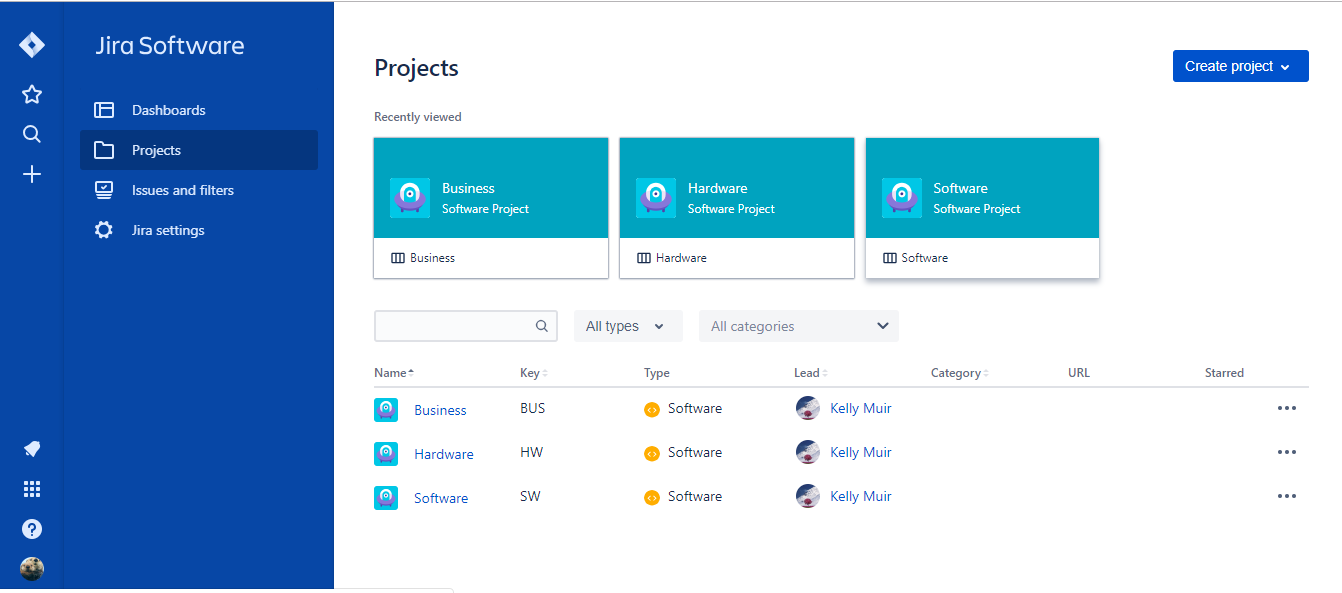
\includegraphics[width=.6\textwidth]{02_09-10/images/jiradash.png}
    \caption{Jira Dashboard}
    \label{fig:jiradash}
\end{figure}

\end{document}